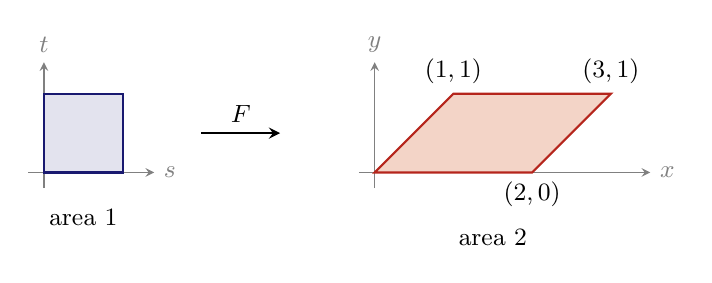
\begin{tikzpicture}[x=1cm,y=1cm,font=\small,>=stealth]
\begin{scope}
\draw[gray,->] (-.2,0)--(1.4,0) node[right] {$s$};
\draw[gray,->] (0,-.2)--(0,1.4) node[above] {$t$};
\fill[MidnightBlue!12] (0,0) rectangle (1,1);
\draw[MidnightBlue,thick] (0,0) rectangle (1,1);
\node[below] at (.5,-.35) {area $1$};
\end{scope}
\draw[->,thick] (2,.5)--node[above] {$F$}(3,.5);
\begin{scope}[shift={(4.2,0)}]
\draw[gray,->] (-.2,0)--(3.5,0) node[right] {$x$};
\draw[gray,->] (0,-.2)--(0,1.4) node[above] {$y$};
\fill[BrickRed!15] (0,0)--(2,0)--(3,1)--(1,1)--cycle;
\draw[BrickRed,thick] (0,0)--(2,0)--(3,1)--(1,1)--cycle;
\node[above] at (1,1) {$(1,1)$};
\node[above] at (3,1) {$(3,1)$};
\node[below] at (2,0) {$(2,0)$};
\node[below] at (1.5,-.6) {area $2$};
\end{scope}
\end{tikzpicture}
